%% examples.tex

%% Example 3.1
In computer graphics, 3D objects can often be parametrized by functions.
Moreover, low to medium accuracy interpolation is usually sufficient to project
satisfactory visual preceptions. In the following example, we use \funappxg to
interpolate the surface of a seashell, leading to a sufficiently accurate
three-dimensional reconstruction.

\begin{figure}[tbh]
  \centering
  \begin{tabular}{cc}
     \includegraphics[width=35mm]{figure/funappxseashell.pdf} 
  & \includegraphics[width=83mm]{figure/seashellsurferror.pdf}
  \\ a)  & b) 
  \end{tabular}
\caption{a) Approximate seashell; b) Error estimation of seashell with tolerance
$0.1$. This figure is reproducible by \texttt{traub\_funappxseashell.m}.}
\label{fig:funappxseashell}
\end{figure}
\begin{exmp}
 
Figure~\ref{fig:funappxseashell}a) is an approximation of a 
seashell portrayed as a parametric surface in 3D. Let $a=-0.2$, $b=0.5$,
$c=0.1$, $n = 2$, $u,v \in [0, 2 \pi]$, and $w(v) =
a\left(1-\frac{v}{2\pi}\right)$. The parametric surface is defined by the
following equations in~\cite{DavEtal05}:
\begin{align*}
x(u,v) & =   \left[ w(v) \left(1+\cos(u)\right) + c\right]\cos(nv),\\
y(u,v) & = \left[w(v) (1+\cos(u)) + c\right] \sin(nv),\\
z(u,v) & = {bv}/{2\pi} + w(v)\sin(u).
\end{align*}
%
\begin{comment}
If a function of two variables $f(x,y)$ can be separated, such as
$$f(x,y)=f_1(x)+f_2(y) \text{ or } f(x,y)=f_1(x)f_2(y),$$ we can apply
\texttt{funappx\_g} directly to $f_1(x)$ and $f_2(y)$. However, $x(u,v)$,
$y(u,v)$, and $z(u,v)$ can not be represented by the form mentioned above.
Instead,
\end{comment}
%We approximate $\sin(x)$ and $\cos(x)$ on the interval $[0,4\pi]$. Denote
Denote $\sinappx(x)$ and $\cosappx (x)$ the approximate functions of $\sin(x)$ and
$\cos(x)$ on the interval $[0,4\pi]$, respectively; and let the resultant
approximants of $x(u,v)$, $y(u,v)$, and $z(u,v)$ be $\hat{x}(u,v)$,
$\hat{y}(u,v)$, and $\hat{z}(u,v)$, respectively.
\begin{comment}
Then we have
\begin{align*}
   \hat{x}(u,v) & =  \left[a\left(1-\frac{v}{2\pi}\right)\left(1+\cosappx(u)\right) + c\right]\cosappx(nv),
\\ \hat{y}(u,v) & = \left[a\left(1-\frac{v}{2\pi}\right)(1+\cosappx(u)) + c\right] \sinappx(nv),
\\ \hat{z}(u,v) & = \frac{bv}{2\pi} + a\left(1-\frac{v}{2\pi}\right)\sinappx(u).
\end{align*}
\end{comment}
Define the overall approximation error measure as
\begin{align*}
\mathscr{E} =  \max\limits_{u,v \in [0, 2 \pi] } & \left\{   |x(u,v)-\hat{x}(u,v)|,\right.
   \left.  |y(u,v)-\hat{y}(u,v)|, 
                                  \ \    |z(u,v)-\hat{z}(u,v)|\right\}.
\end{align*}
Even if we set the error tolerance $\abstol$ to be as big as $0.1$ for computing
$\sinappx$ and $\cosappx$, we can still obtain a much diminished error
$\mathscr{E}\approx 9 \times 10^{-4}$; see the error plot in
Figure~\ref{fig:funappxseashell}b). The reconstructed surface in
Figure~\ref{fig:funappxseashell}a) is very similar to the original seashell
image.
\end{exmp}

In digital animation, frames of images are produced to represent movements of
objects over small discrete time. To automatically insert additional frames between 
two consecutives frames for better visual effects, temporal
interpolation can often be applied to estimate an object's positions by using
parametric curves that represent its trajectory in 3D as $(x(t), y(t), z(t))$,
where each Cartesian coordinate in space is parametrized by time $t$. We refer
readers to Example~5 in \cite[Section 3.6]{Din15a} for an illustration.

%% Example 3.2

The next example showcases the merits and demerits of our algorithm and an
existing method for high-accuracy function approximation.

\begin{exmp}
Chebfun~\cite{TrefEtal15a} is a MATLAB toolbox known for using Chebyshev
polynomial basis for approximating given functions to machine precision
($\approx 10^{-15}$). In this example, we show that it is challenged by~$f_3$
defined in Section~\ref{sec:cone}. Around $x=0$ and $x=0.2$, some pointwise
errors of the piecewise Chebyshev interpolant spike to more than $10^{-5}$ as
shown in Figure~\ref{f3fig}a). Regretably Chebfun did not issue any warning
about the inaccurate representation in this case. In contrast, the errors of the
piecewise linear interpolant from \funappxg{} are uniformly below $10^{-14}$.
Nonetheless the time taken by \funappxg{} was close to 7 seconds for such an 
accurate approximation.

\begin{figure}[t]
\centering
\begin{tabular}{cc}
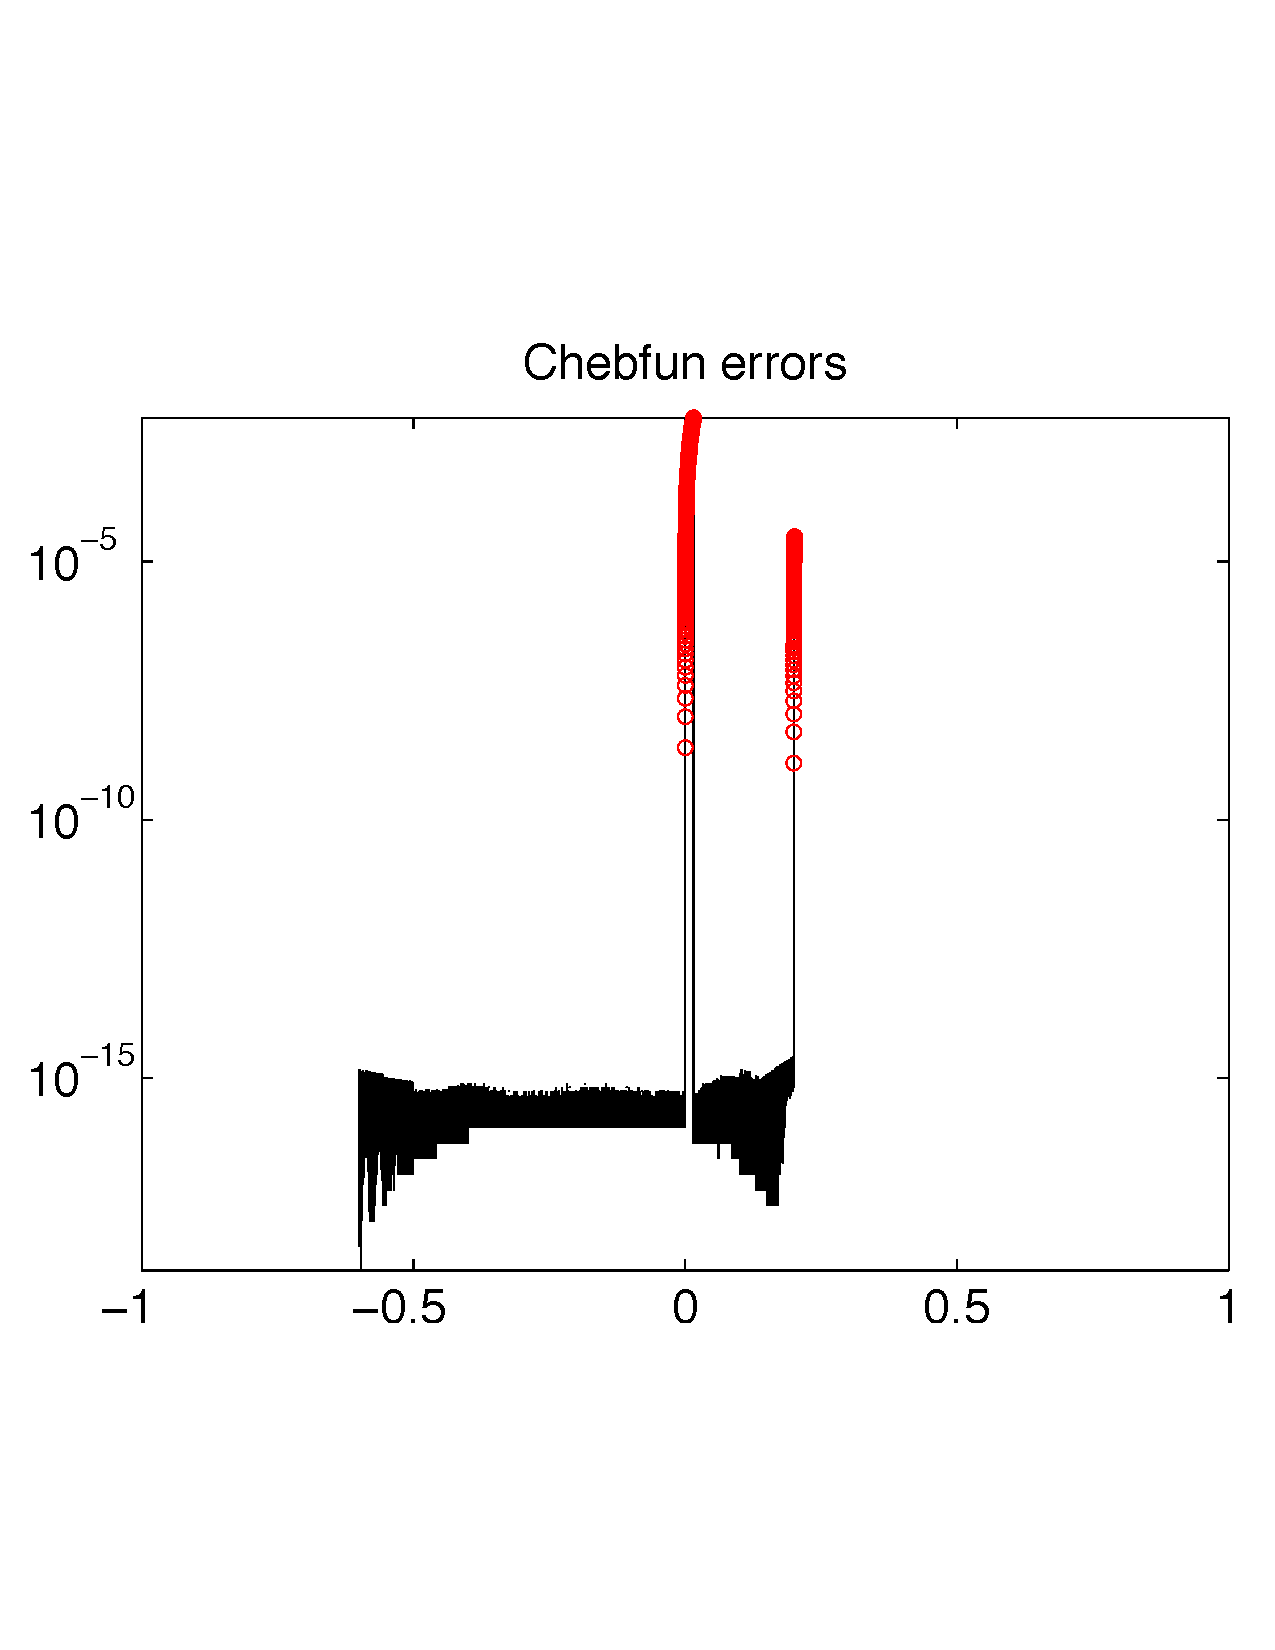
\includegraphics[width=5.9cm]{figure/chebfun_errors.pdf} \hspace{-2ex} &
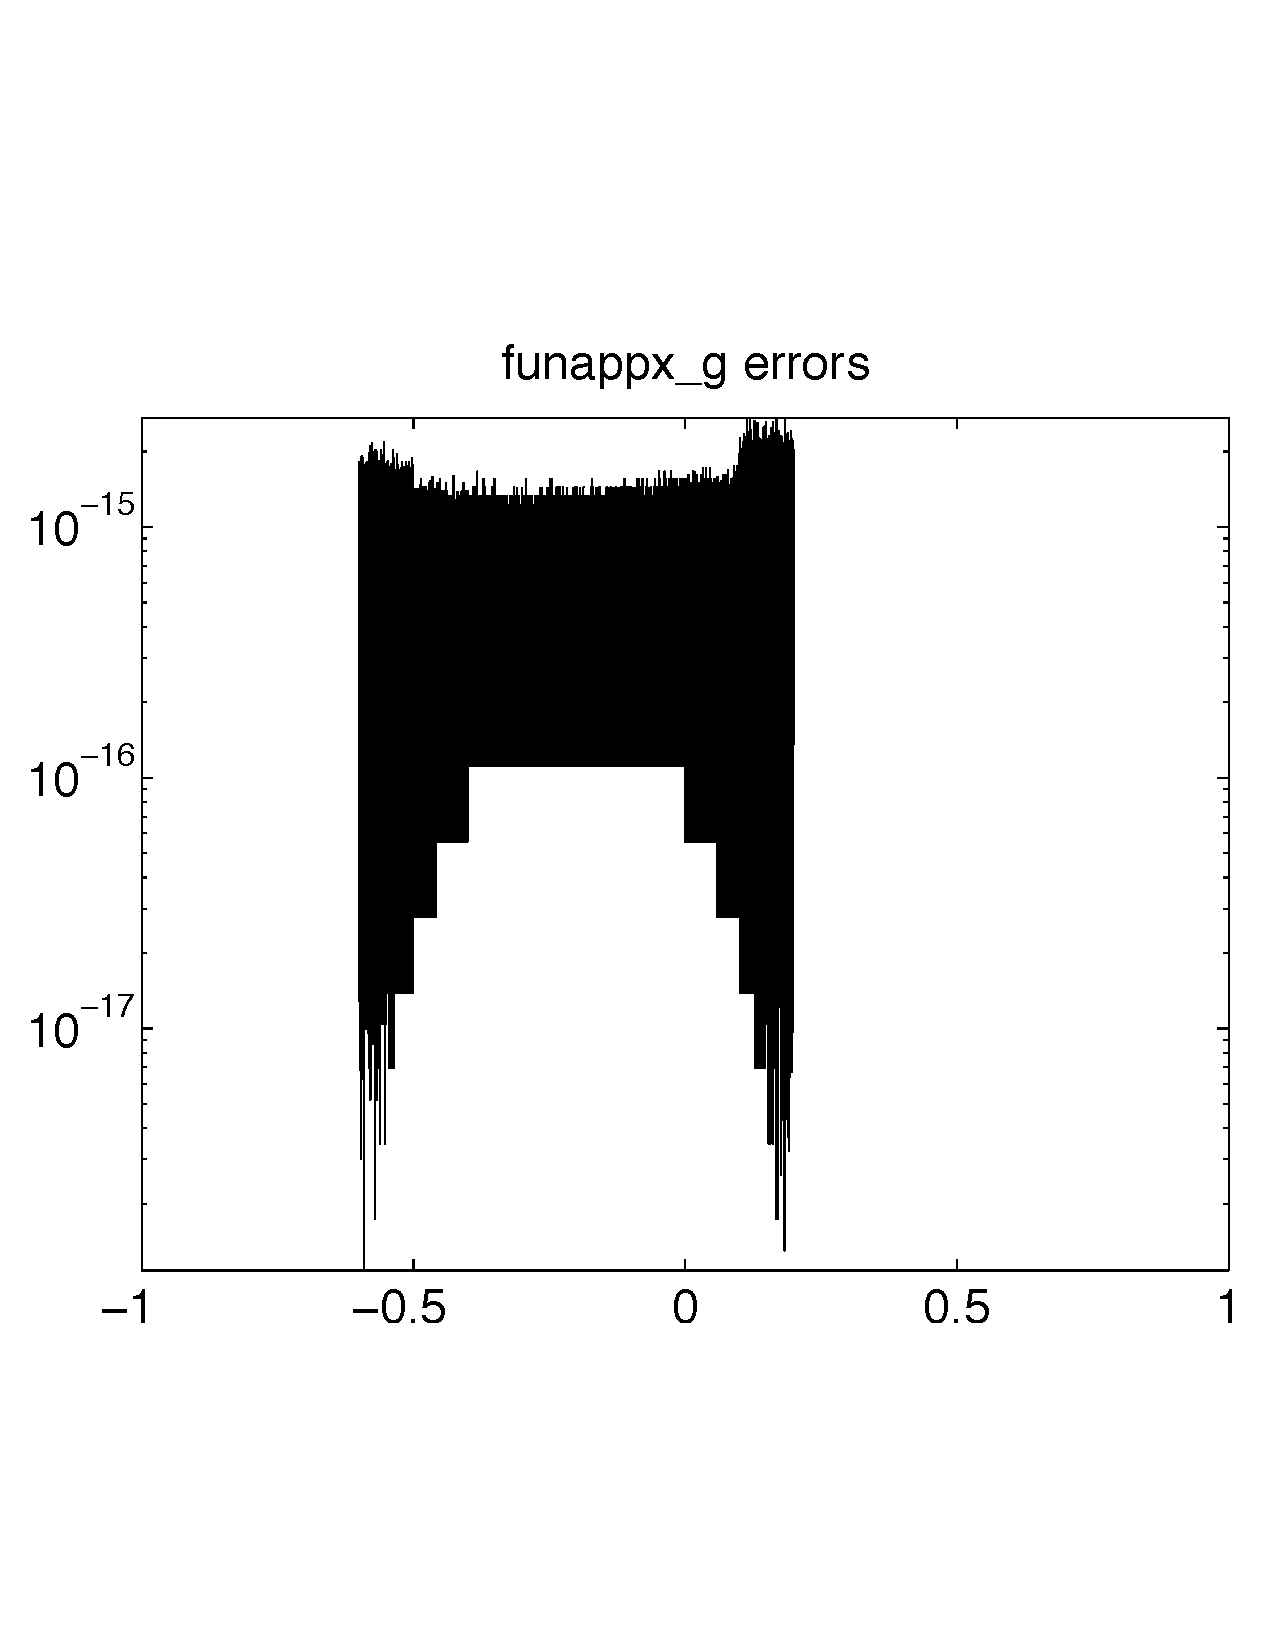
\includegraphics[width=5.9cm]{figure/funappx_g_errors.pdf}
\\ a) & b)
\end{tabular}
\caption{Approximating $f_3(x)$ with errors of interpolants returned from a)
Chebfun and b) \funappxg. This figure is reproducible by
\texttt{cf\_chebfun.m}.}
\label{f3fig}
\end{figure}
\end{exmp}

\begin{comment}
Our algorithm is readily extensible to the following complex-valued function.
\begin{exmp}
This example is taken from MATLAB's documentation for \texttt{interp1}. 
Define the complex valued function
$v(x) = 5x + x^2 i$ for $x \in [1,10]$.  It is clear that the real part of $v$ 
is $5x$ and the imaginary part is $x^2$. We could  
apply \funappxg  to approximate the two parts separately. However, it is unnecessary.

\end{exmp}
\end{comment}

\begin{exmp}
In this example, we consider the function $f_4(x) = sin(10 \pi x^4) + x$, which is increasing oscillating over the interval $[0,2]$.
We use \funappxg, \funming, and \integralg to approximate the function, locate its global minimum, and estimate its integral with $\abstol = 10^{-8}$.
With $1,972,359$ points, \funappxg can approximate $f_4$ uniformly accurate as shown in Figure~\ref{f4fig}(a).
The true global minimum is $(0.6212340312, -0.3782149854)$ and the absolute approximation error of \funming using $n=2,022,621$ points is      
$(1.4\times 10^{-7}, 4.7\times 10^{-11})$. The integral 
$\int_{0}^{2} f_4 (x) dx = 2.145517314$ and the approximation error of \integralg is $4.7\times10^{-10}$ using $4,965,641$ points.

\begin{figure}[bt]
\centering
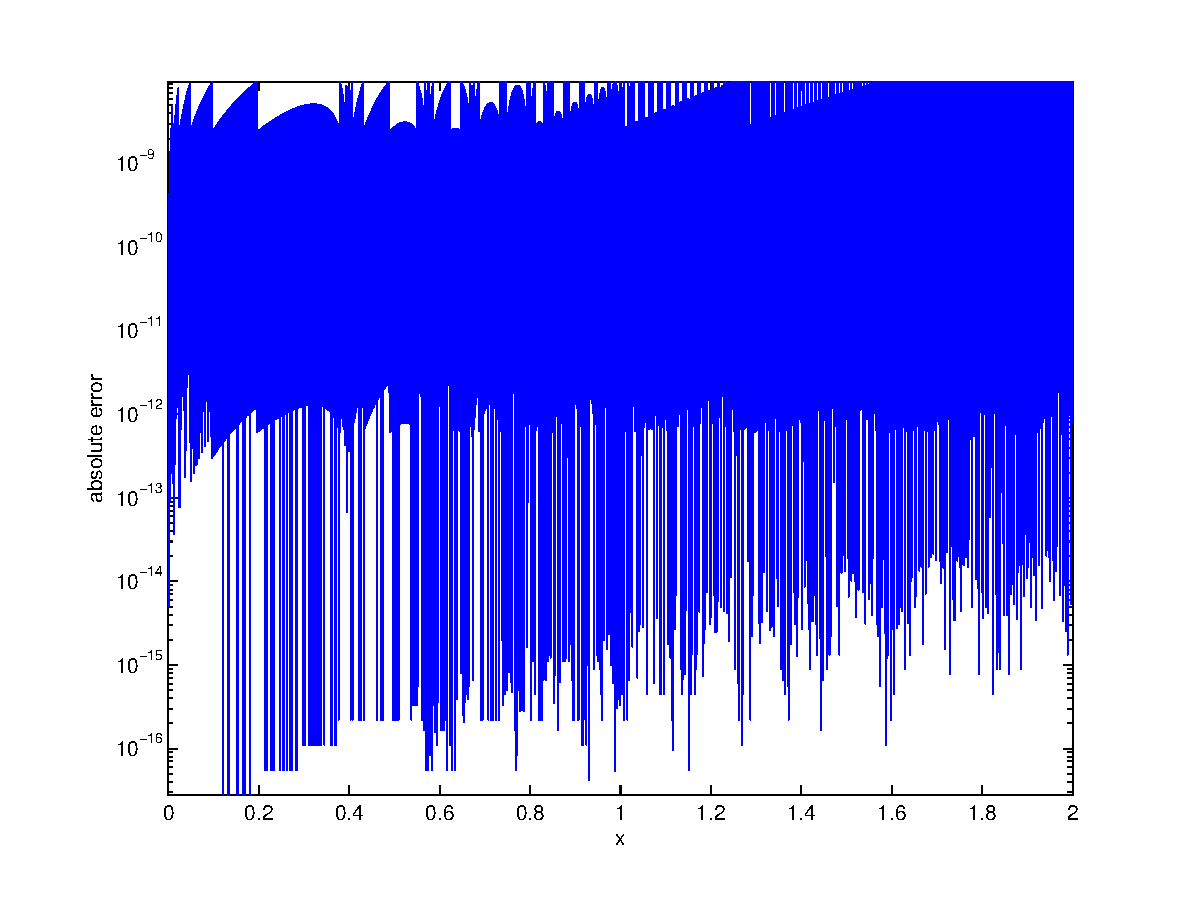
\includegraphics[width=6.2cm]{figure/f4_funappx_error.eps} \hspace{-5ex}
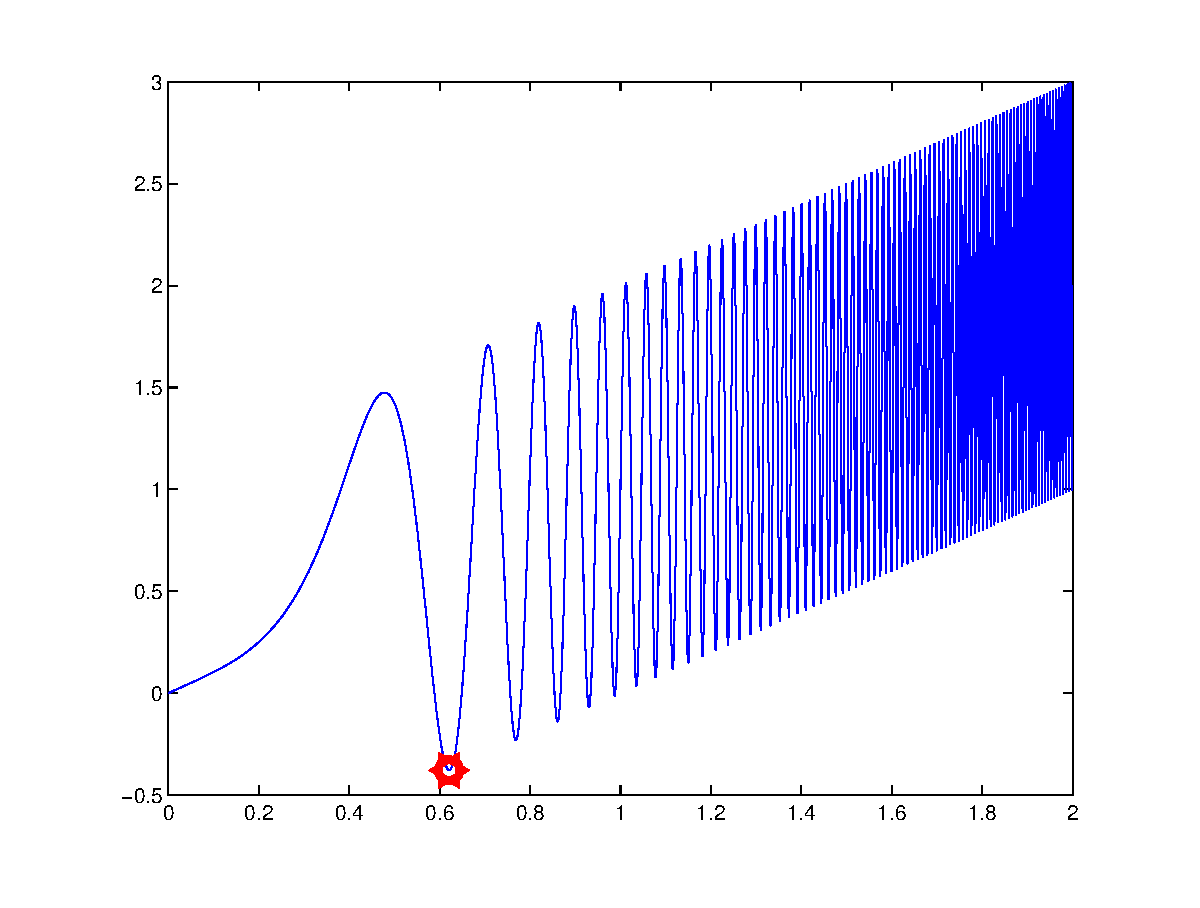
\includegraphics[width=6.2cm]{figure/f4_funmin_g.eps}
\caption{The example $f_4$ with errors of interpolants from \funappxg (left) and minimum found by \funming (right).}
\label{f4fig}
\end{figure}
\end{exmp}
